\section{Logic}

As we are dealing with a \textbf{thin client | fat server} model, figure 1 outlines the general idea behind communication required for the game of Spades. The client will initialize the process with a login request. After which \textit{(assuming success)} the server will reply and grant the client access to the game lobby. The client will either attempt to join a game or instantiate a new one. After the game is fully set up the game initializes a loop handing the client - server for the remainder of the game. The server sends the state of the game along with a list of legal moves. The client will reply. This process will continue until the game is either interrupted or completed. After which, the server grants access to the lobby.  	

\begin{figure}
		% Center the figure.
		\begin{center}
		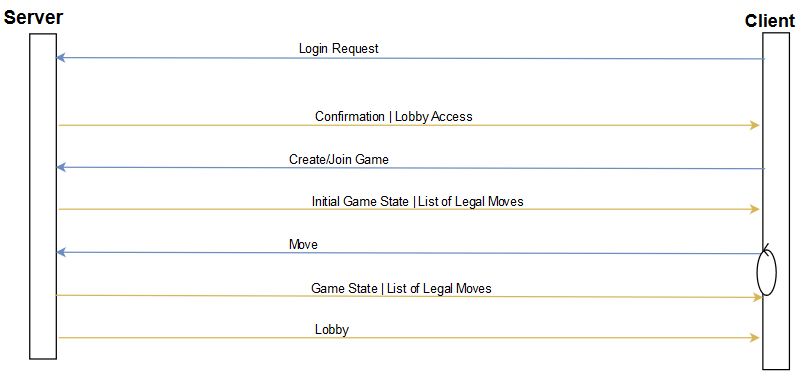
\includegraphics{graphics/clientServer}
		% Create a subtitle for the figure.
		\caption{Server - Client model for spades.}
		% Define the label of the figure. It's good to use 'fig:title', so you know that the label belongs to a figure.
		\label{Figure 1}
		\end{center}
	\end{figure}
	
	\begin{figure}
		% Center the figure.
		\begin{center}
		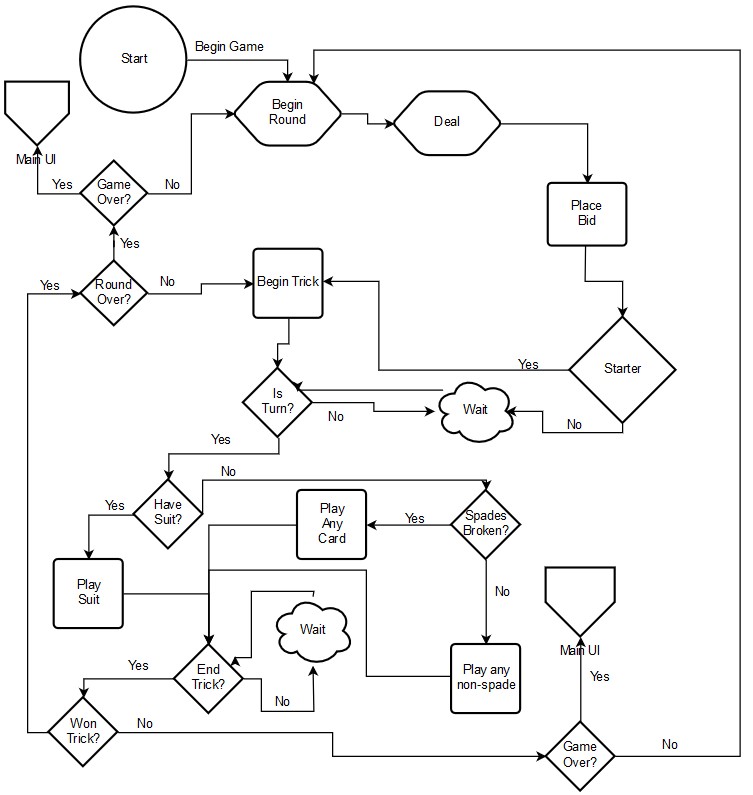
\includegraphics{graphics/logicDiagram}
		% Create a subtitle for the figure.
		\caption{Activity diagram for spades.}
		% Define the label of the figure. It's good to use 'fig:title', so you know that the label belongs to a figure.
		\label{Figure 1}
		\end{center}
	\end{figure}
	